\documentclass[10pt,twocolumn]{article}
\usepackage[final]{neurips_2024}
\usepackage[T1]{fontenc}
\usepackage[utf8]{inputenc}
\usepackage{booktabs}
\usepackage{graphicx}
\usepackage{amsmath}
\usepackage{amssymb}
\usepackage{subcaption}
\usepackage{enumitem}
\setlist[itemize]{leftmargin=1.2em, itemsep=0.15em, topsep=0.2em}
\captionsetup{font=small}
\captionsetup[subfigure]{skip=2pt}
\makeatletter
\setlength{\@fptop}{0pt}
\setlength{\@fpbot}{0pt plus 1fil}
\setlength{\@fpsep}{12pt plus 0fil}
\makeatother
\setlength{\textfloatsep}{8pt plus 2pt minus 2pt}
\setlength{\floatsep}{8pt plus 2pt minus 2pt}

\title{Examining Generalization in Procgen with Simple Temporal and Visual Architecture Changes}
\author{%
{\small
\begin{tabular}{@{}c@{\hspace{1em}}c@{\hspace{1em}}c@{}}
Elya Renom & William Potter & Tong Wu \\
McGill University & McGill University & McGill University \\
\texttt{261094604} & \texttt{261072144} & \texttt{261224077}
\end{tabular}} \\[0.6em]
{\small COMP 579 Project, McGill University, Winter 2026}
}

\begin{document}
\maketitle

\begin{abstract}
We study generalization in reinforcement learning using the Procgen benchmark, where an agent is trained on one set of procedurally generated levels and evaluated on a disjoint held-out set. Our baseline is Proximal Policy Optimization (PPO), and we compare it to two simple architecture changes motivated by recent Procgen work: four-frame stacking and four-frame stacking combined with a deeper convolutional encoder. We evaluate three games with distinct visual and control demands: CoinRun, Dodgeball, and StarPilot. Across a one-million-step, five-seed setting, the results show that generalization gaps do appear, but the effect of architectural changes is strongly game-dependent. Frame stacking is most helpful on CoinRun, the larger CNN is most helpful on Dodgeball, and the baseline PPO remains strongest on StarPilot at this compute budget. The project therefore supports the broader claim that representation choices matter for transfer, while also showing that simple changes are not universally beneficial.
\end{abstract}

\section{Introduction}
A recurring difficulty in reinforcement learning is that good training performance does not necessarily imply good transfer to new situations. Agents can memorize narrow regularities in their training environments, especially when those environments are visually rich and only partially explored. This makes generalization an important empirical question even when the optimization algorithm itself is stable.

The Procgen benchmark was designed to make this question measurable: agents train on a finite set of procedurally generated levels and are then tested on disjoint unseen levels from the same game family \citep{cobbe2020procgen}. Unlike small tabular control problems, Procgen combines sequential decision making, visual perception, and out-of-distribution evaluation in one benchmark. This makes it attractive for controlled empirical study because it gives a clear train/test split, intuitive task differences across games, and plots that can be interpreted directly.

Our project asks a narrow version of the generalization problem: if PPO is held fixed, can simple changes to the input representation and visual encoder improve performance on unseen Procgen levels? Following \citet{jesson2024procgen}, we compare three variants: standard PPO, PPO with frame stacking, and PPO with frame stacking plus a larger CNN. The initial design used CoinRun, Heist, and StarPilot, but we replaced Heist with Dodgeball because Heist remained effectively inactive at our compute budget, making it a poor use of limited CPU training time. The resulting study is therefore less a full reproduction of the modern Procgen scale regime and more a controlled analysis of what can already be learned from a modest 1M-step setting.

\section{Background}
\textbf{PPO.} PPO is a policy-gradient method that updates a parameterized policy using a clipped surrogate objective designed to improve stability over naive policy optimization \citep{schulman2017ppo}. PPO fits naturally into the actor-critic family: the policy selects actions, while a value function provides a lower-variance training signal. In our project, PPO is the learning algorithm held constant across all variants.

\textbf{Procgen generalization.} Procgen defines a family of visually diverse games in which levels are generated algorithmically rather than stored explicitly \citep{cobbe2020procgen}. This enables a direct separation between \emph{seen} training levels and \emph{unseen} test levels. We report seen-level return, unseen-level return, and the generalization gap
\[
\text{gap} = \text{seen return} - \text{unseen return}.
\]
A positive gap indicates that the agent performs better on the levels it trained on, which is the usual signature of overfitting.

\textbf{Architecture changes.} The main additions beyond the baseline are the representation-side modifications. Frame stacking concatenates multiple recent frames so that velocity and short-term motion can be inferred directly from the input. This is particularly relevant when a single frame under-specifies the state. The larger CNN increases encoder depth and capacity, which can help when the visual scene is cluttered or when task-relevant features are harder to extract. The risk is that higher-capacity encoders may also become more sample-hungry, especially under a small compute budget \citep{jesson2024procgen}.

\section{Methodology}
We trained three variants on three Procgen games. The baseline \texttt{ppo} receives a single RGB frame and uses the default Stable-Baselines3 \texttt{NatureCNN}. The \texttt{ppo\_frame\_stack} variant receives four stacked RGB frames but keeps the same encoder. The \texttt{ppo\_frame\_stack\_large\_cnn} variant also receives four frames, but replaces the default encoder with a custom four-layer CNN with channel progression 64-128-128-128. Implementation was done in Stable-Baselines3 \citep{raffin2021sb3} using a single-file training pipeline.

The environments are CoinRun, Dodgeball, and StarPilot. CoinRun is a relatively simple platformer whose dynamics make velocity information important. Dodgeball contains more spatial clutter and projectile interactions. StarPilot is a scrolling shooter with denser visual motion and less forgiving control. All runs use Procgen's \texttt{easy} distribution mode. Training levels are generated from \texttt{start\_level}=0 with 200 levels, and test levels are generated from \texttt{start\_level}=10000 with 200 levels, so there is no overlap between seen and unseen sets.

For the full experiment we used five seeds, 1M environment steps per run, evaluation every 100k steps, 20 evaluation episodes per checkpoint, and 8 parallel environments. Hyperparameters closely follow the default Procgen PPO setup: learning rate $2.5\times 10^{-4}$, $n\_\text{steps}=256$, batch size 256, 4 PPO epochs, $\gamma=0.999$, $\lambda=0.95$, clip range 0.2, entropy coefficient 0.01, value coefficient 0.5, and max gradient norm 0.5. We aggregate all metrics across seeds, visualize the full learning curves, and compare final unseen return and final generalization gap with mean \(\pm\) standard deviation.

Table~\ref{tab:variants} summarizes the intended role of each architecture. The point of the design is not to introduce a radically new algorithm, but to isolate two plausible sources of better transfer while keeping the optimization rule fixed. This makes the experiment easier to interpret than a comparison between entirely different RL methods.

\begin{table}[h]
\centering
\small
\begin{tabular}{p{0.18\columnwidth}p{0.16\columnwidth}p{0.16\columnwidth}p{0.38\columnwidth}}
\toprule
Variant & Temporal input & Encoder size & Expected effect \\
\midrule
PPO & One frame & Default CNN & Stable baseline, but limited motion information \\
Frame stack & Four frames & Default CNN & Better short-horizon dynamics, possible capacity bottleneck \\
Frame stack + large CNN & Four frames & Deeper CNN & Better motion and richer visual features, but more sample-hungry \\
\bottomrule
\end{tabular}
\caption{Conceptual role of the three model variants.}
\label{tab:variants}
\end{table}

\section{Experimental Results}
Figures~\ref{fig:coinrun}--\ref{fig:starpilot} summarize the learning curves and final metrics for each game. The central result is that there is no single architecture that dominates across games.

\begin{figure*}[!t]
    \centering
    \begin{subfigure}[t]{0.49\textwidth}
        \centering
        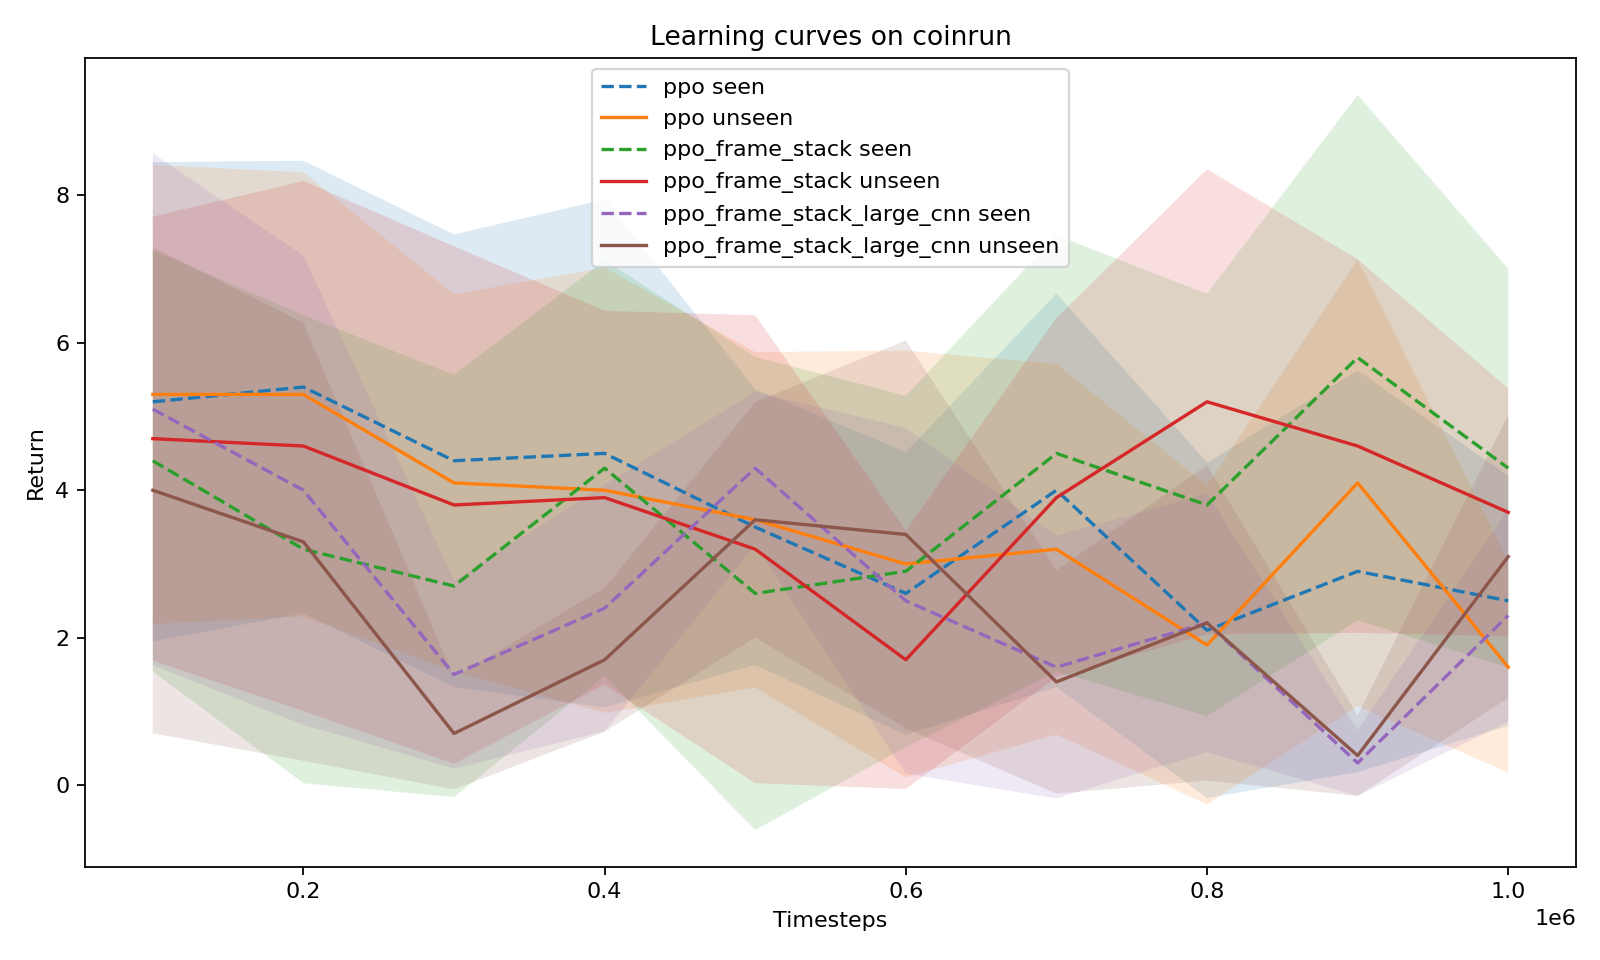
\includegraphics[width=\linewidth,trim=8 8 8 8,clip]{figures/learning_curves_coinrun.png}
        \caption{Learning curves}
    \end{subfigure}%
    \hfill
    \begin{subfigure}[t]{0.49\textwidth}
        \centering
        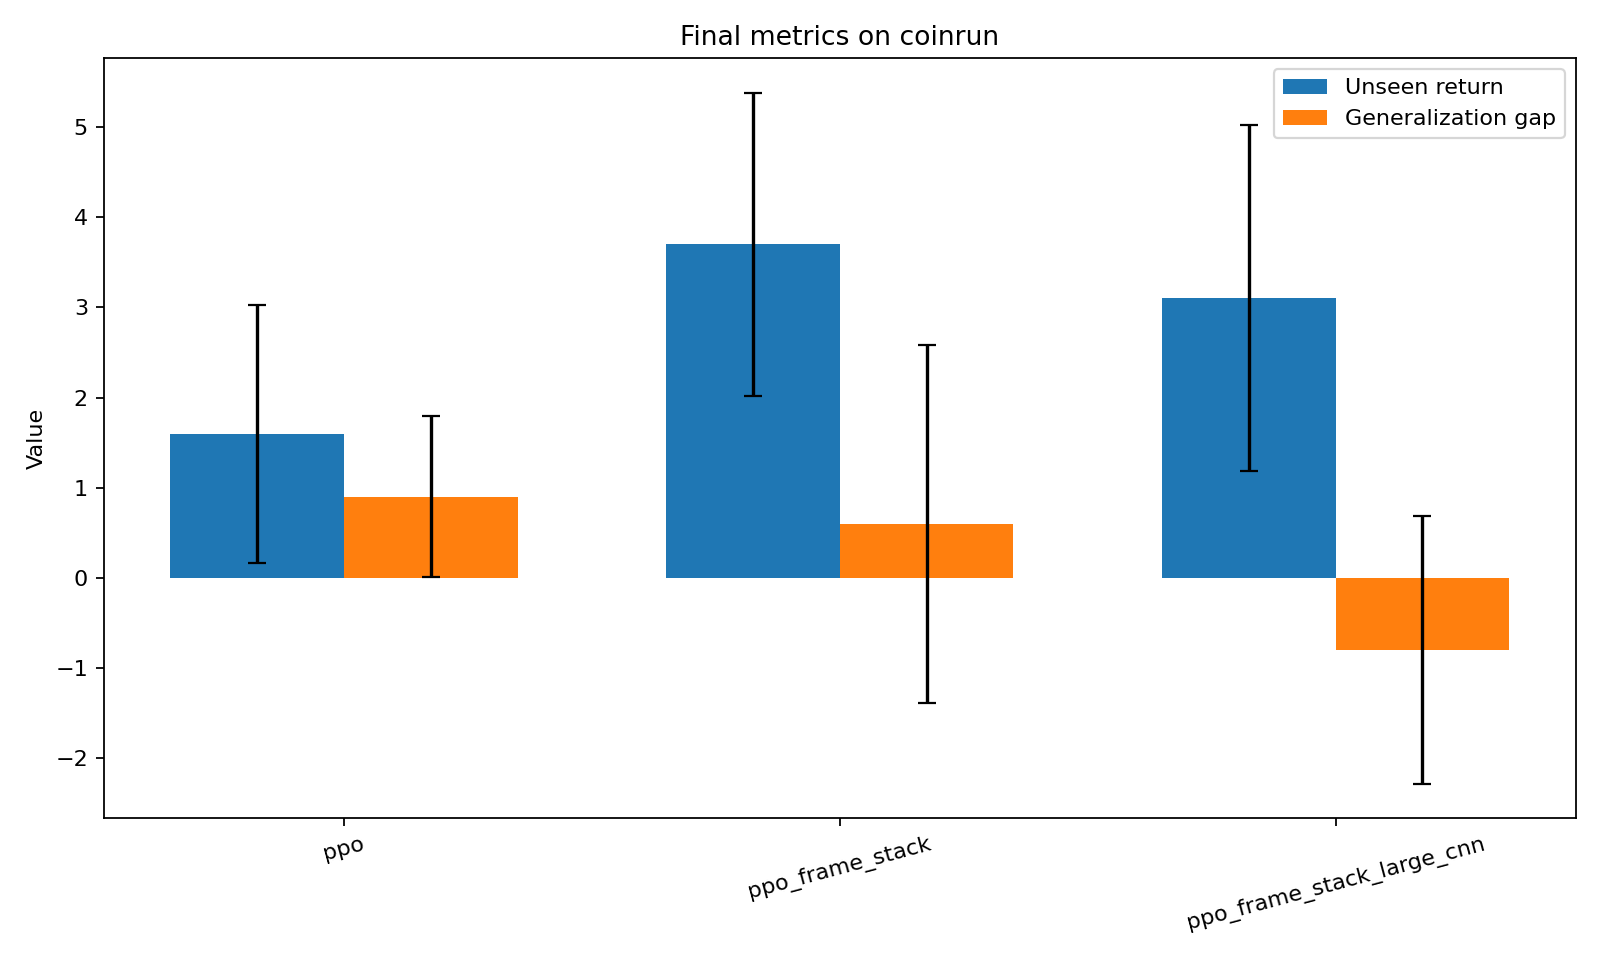
\includegraphics[width=\linewidth,trim=8 8 8 8,clip]{figures/final_bars_coinrun.png}
        \caption{Final metrics}
    \end{subfigure}
    \caption{CoinRun. Left: mean seen (dashed) and unseen (solid) returns over training, shaded regions show standard deviation across five seeds. Right: final unseen return and final generalization gap per variant.}
    \label{fig:coinrun}
\end{figure*}

\textbf{CoinRun.} CoinRun is the clearest case where frame stacking helps. Its final unseen return is $3.7 \pm 1.7$, compared with $1.6 \pm 1.4$ for baseline PPO and $3.1 \pm 1.9$ for the larger CNN. Its estimated generalization gap is also smaller than the baseline's, at $+0.60 \pm 1.98$ versus $+0.90 \pm 0.89$, while the large-CNN variant has a negative estimated gap of $-0.80 \pm 1.48$. This is consistent with the task structure: jumps and obstacle timing depend strongly on short-horizon motion cues, which a single frame cannot represent well. The most important qualitative feature, however, is instability. All CoinRun variants show non-monotonic learning, with performance peaking well before the final checkpoint in several runs. As a result, final-only comparisons understate how much competence was reached during training.

\begin{figure*}[!t]
    \centering
    \begin{subfigure}[t]{0.49\textwidth}
        \centering
        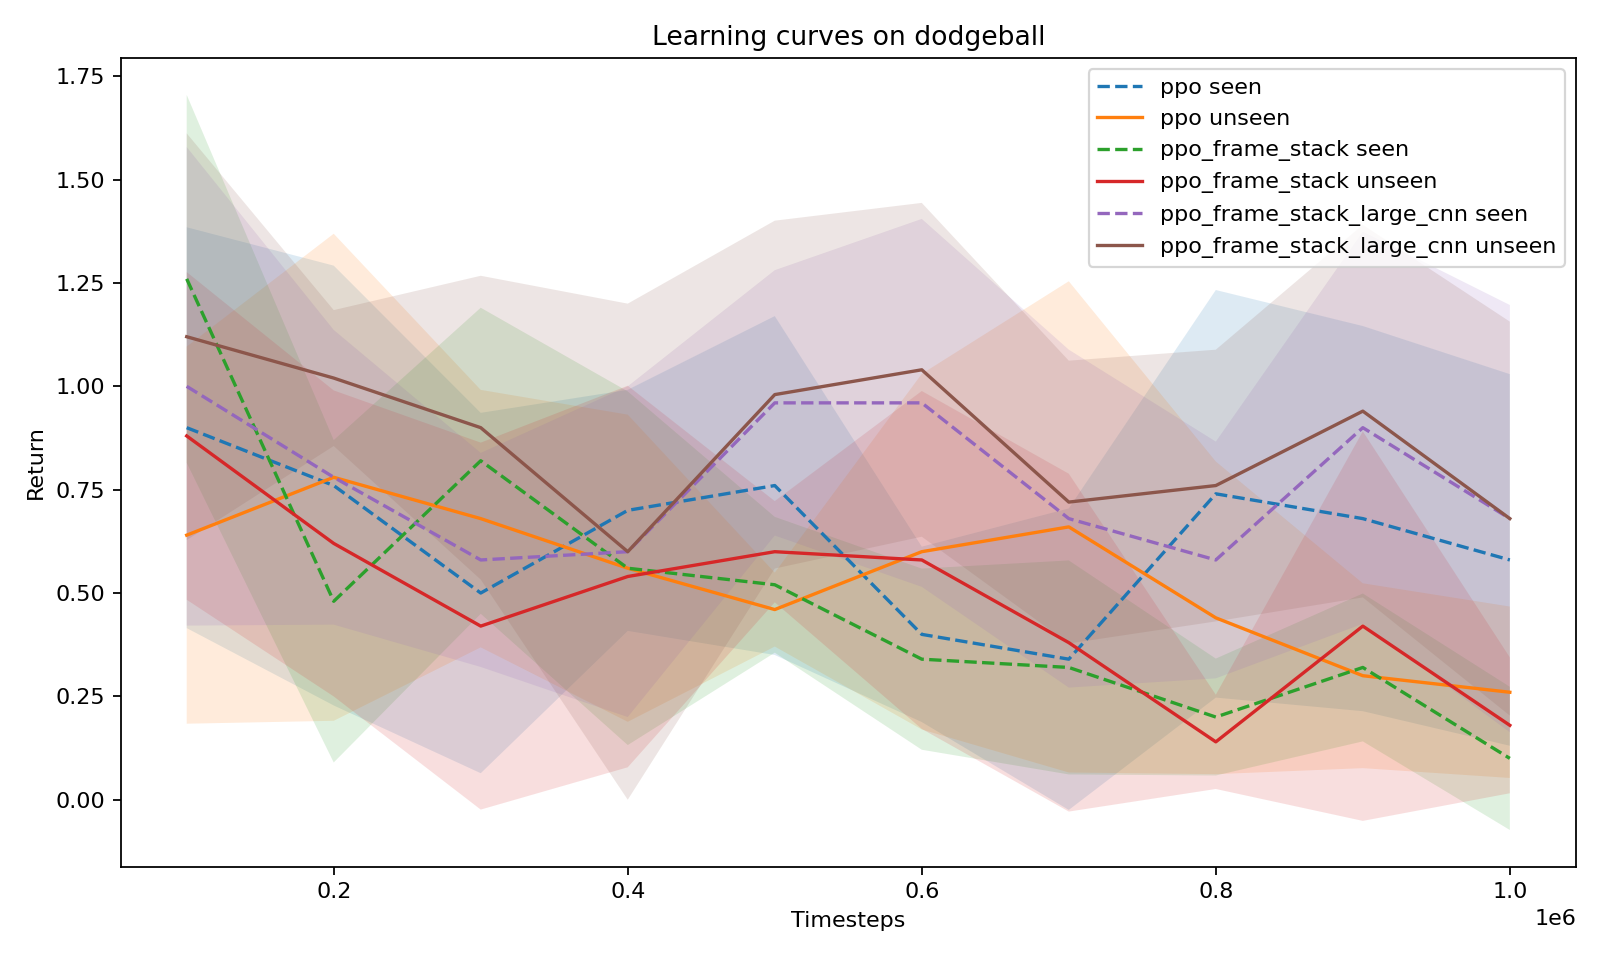
\includegraphics[width=\linewidth,trim=8 8 8 8,clip]{figures/learning_curves_dodgeball.png}
        \caption{Learning curves}
    \end{subfigure}%
    \hfill
    \begin{subfigure}[t]{0.49\textwidth}
        \centering
        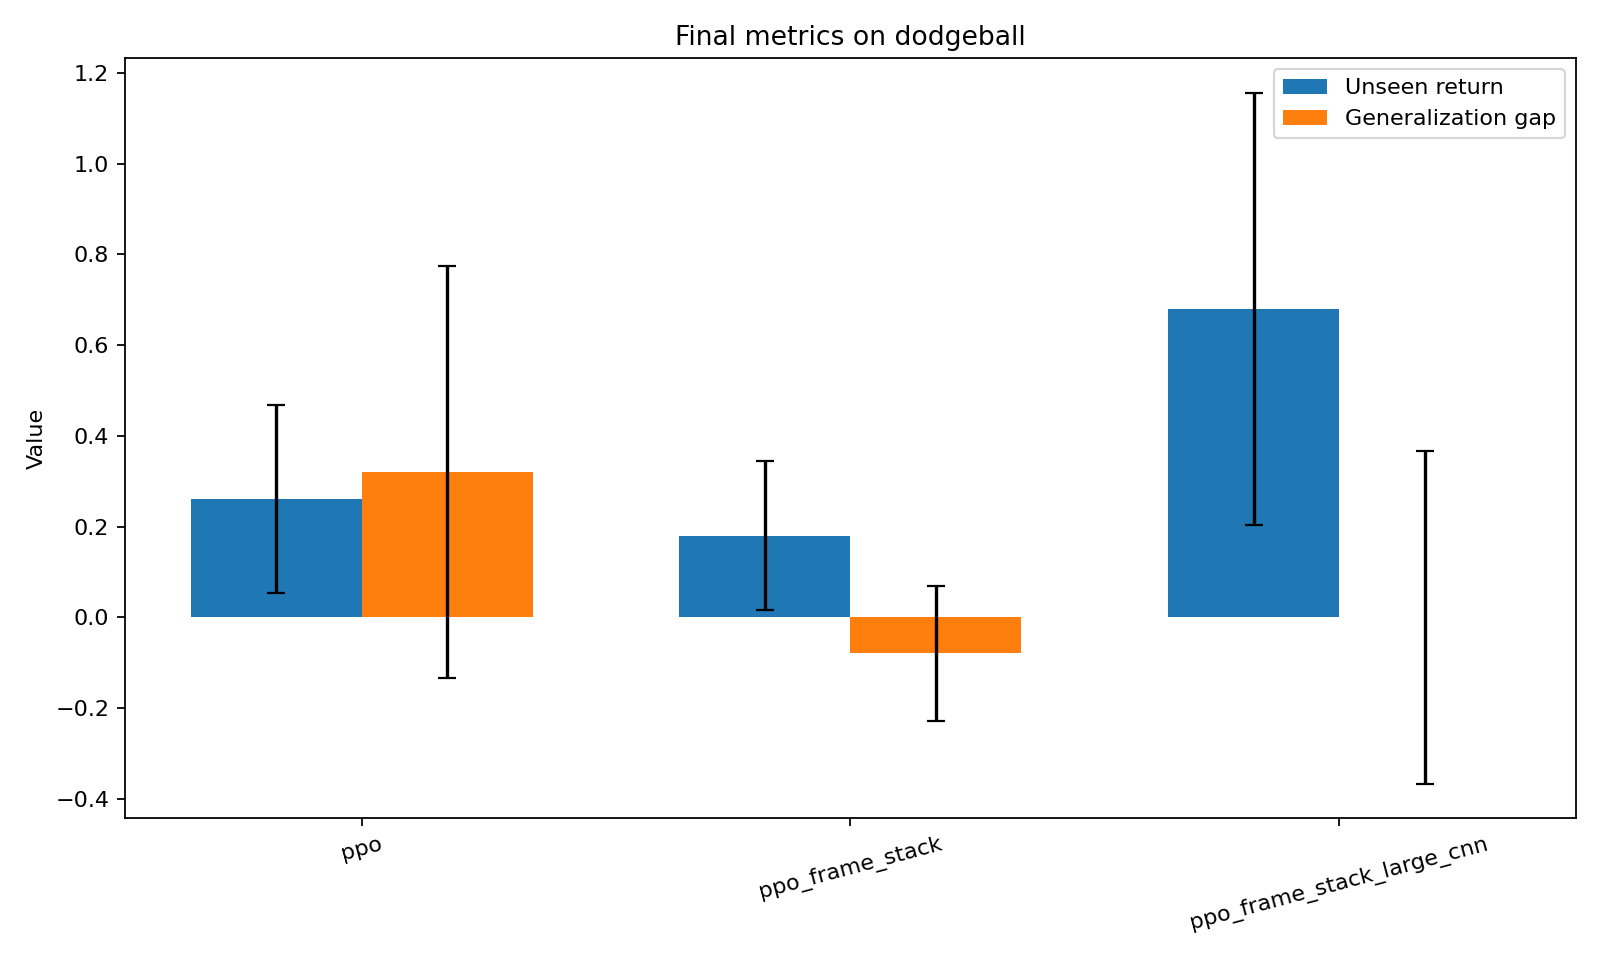
\includegraphics[width=\linewidth,trim=8 8 8 8,clip]{figures/final_bars_dodgeball.png}
        \caption{Final metrics}
    \end{subfigure}
    \caption{Dodgeball. Left: mean seen (dashed) and unseen (solid) returns over training, shaded regions show standard deviation across five seeds. Right: final unseen return and final generalization gap per variant.}
    \label{fig:dodgeball}
\end{figure*}

\textbf{Dodgeball.} Dodgeball shows the opposite pattern. Frame stacking alone is not clearly helpful: its final unseen return is $0.18 \pm 0.16$, slightly below the baseline's $0.26 \pm 0.21$. The deeper encoder achieves the strongest final unseen return, $0.68 \pm 0.48$, and yields the smallest estimated gap ($\approx 0 \pm 0.37$) whereas the baseline retains a positive gap of $0.32 \pm 0.45$. A plausible interpretation is that Dodgeball is more visually complex than CoinRun, so adding temporal channels without increasing encoder capacity overloads the default CNN, whereas the larger encoder can make use of the richer input.

\begin{figure*}[!t]
    \centering
    \begin{subfigure}[t]{0.49\textwidth}
        \centering
        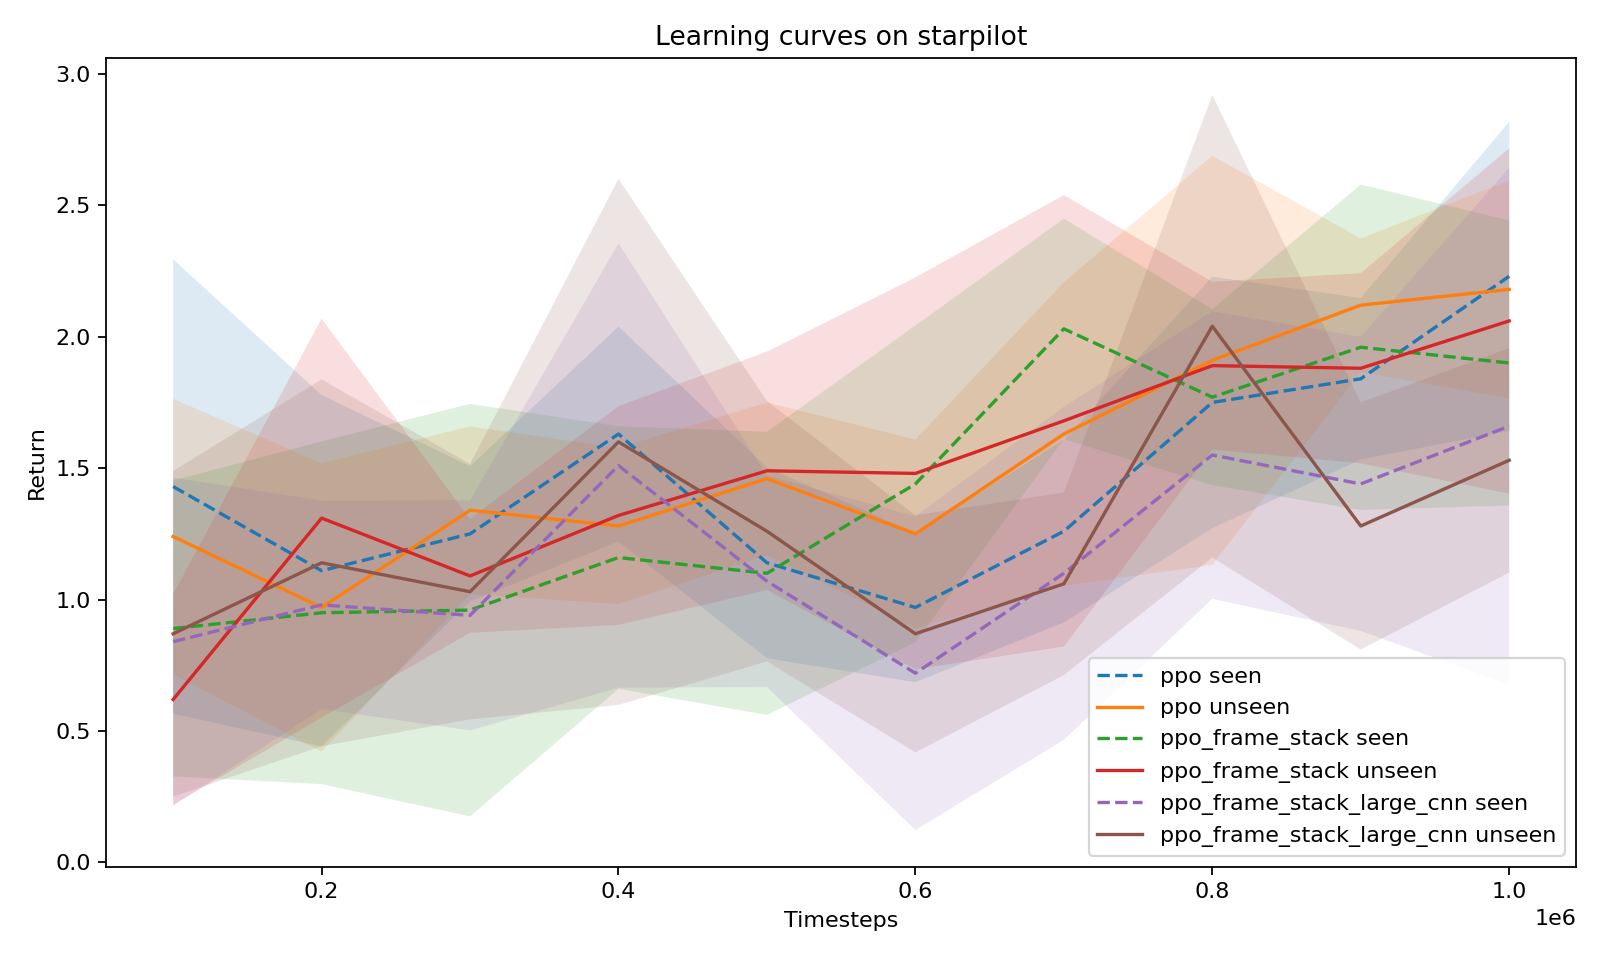
\includegraphics[width=\linewidth,trim=8 8 8 8,clip]{figures/learning_curves_starpilot.png}
        \caption{Learning curves}
    \end{subfigure}%
    \hfill
    \begin{subfigure}[t]{0.49\textwidth}
        \centering
        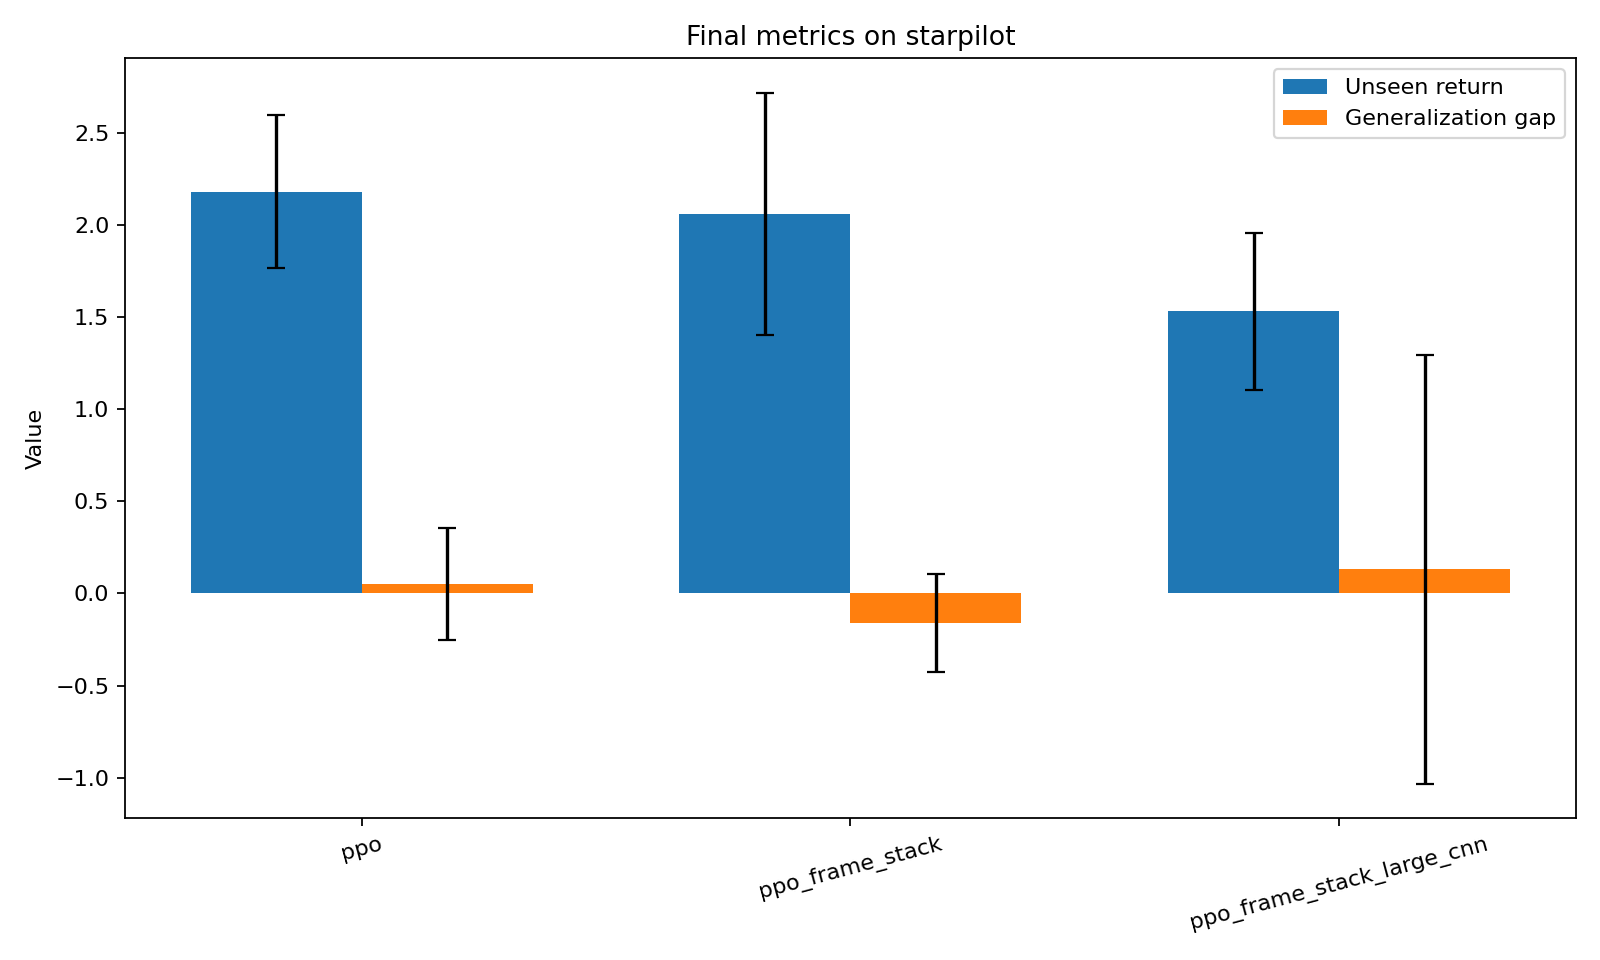
\includegraphics[width=\linewidth,trim=8 8 8 8,clip]{figures/final_bars_starpilot.png}
        \caption{Final metrics}
    \end{subfigure}
    \caption{StarPilot. Left: mean seen (dashed) and unseen (solid) returns over training, shaded regions show standard deviation across five seeds. Right: final unseen return and final generalization gap per variant.}
    \label{fig:starpilot}
\end{figure*}

\textbf{StarPilot.} On StarPilot, the simplest baseline remains strongest at this budget, with a final unseen return of $2.18 \pm 0.41$. Frame stacking is competitive at $2.06 \pm 0.66$ but not clearly better, while the larger CNN lags behind at $1.53 \pm 0.43$. All three variants have near-zero gaps ($0.05 \pm 0.30$, $-0.16 \pm 0.27$, and $0.13 \pm 1.16$ respectively), so the ranking is driven by absolute competence rather than transfer. This suggests that the larger model is under-trained rather than intrinsically bad: StarPilot appears to require either more data or more compute before the additional capacity pays off, and under a 1M-step budget the simpler encoder is easier to optimize.

\section{Discussion}
\textbf{Across-game interpretation.} Two broader conclusions follow. First, the measured generalization gaps are real but generally modest relative to the seed variance. Even when a gap is positive, the error bars overlap substantially in several settings. Second, near-zero or negative estimated gaps should be interpreted cautiously. In this project they are consistent with reduced overfitting, but they are also compatible with underfitting, noise, or unstable learning dynamics. Overall, the experiment supports the methodological claim that Procgen can expose transfer differences, but at 1M steps it does not provide a decisive ranking of these architectures.

\textbf{Scope of the analysis.} Consistent with the controlled-analysis framing of the introduction, our claims are about what can be observed at a 1M-step budget rather than about the asymptotic behaviour of each architecture. The experiment shows that representation choices do shift unseen-level performance, and that these shifts are not uniform across environments. It also makes clear the limits of small-compute analysis in RL: the literature typically reports sharper separations once training extends much further, while our curves still show obvious signs of incomplete convergence, most visibly when a model's best checkpoint is not its last one.

\textbf{Why final metrics can be misleading.} The learning-curve plots matter as much as the final bar charts. If we looked only at the final unseen return, we might conclude that one architecture is simply superior or inferior. The trajectory plots show something more nuanced: some variants learn earlier and then plateau, while others spike and collapse. For CoinRun in particular, the ranking depends on whether we care about best achieved performance or end-of-training performance. This is an important lesson for RL evaluation more generally, because optimization instability can masquerade as poor generalization if only the final checkpoint is reported.

\textbf{Main limitations.} Our conclusions are constrained by three practical issues. First, the compute budget is small relative to common Procgen studies. Second, evaluation variance remains high even with five seeds, especially for sparse or partially solved games. Third, we changed one of the original tasks, replacing Heist with Dodgeball, so the final study should be interpreted as a revised experimental design rather than a full three-game reproduction of the initial plan. None of these limitations invalidate the results, but they do narrow the strength of the claims we can responsibly make.

\section{Conclusion and Future Work}
This project shows that simple architectural changes can affect Procgen transfer, but not in a uniform way. Frame stacking improves the most motion-sensitive game in our set, the larger CNN helps the most visually cluttered one, and the baseline remains strongest when additional capacity cannot be fully trained. The results therefore support a nuanced conclusion: representation matters, but the right representation depends on the game and the available compute.

The clearest next step is scale. The strongest limitation of our study is that 1M steps is enough to observe trends, but not enough to cleanly separate under-training from genuine generalization improvements. Extending the budget to 5M or 25M steps would make the comparison much sharper. Other interesting extensions include adding Heist back once sufficient compute is available, evaluating intermediate-checkpoint best models instead of only the final checkpoint, testing regularization methods such as stronger data augmentation, and comparing these simple modifications with larger-scale architectural improvements from more recent Procgen work.

\section{Contributions and Acknowledgements}
Elya Renom led project framing, implemented the main training pipeline, handled the environment compatibility issues on Apple Silicon, and produced the core experimental runs. Tong Wu and William Potter contributed to debugging, literature review, result analysis, figure discussion, and producing the project video. All team members participated in shaping the research question and reviewing the final report.

We thank the authors and maintainers of Procgen, Stable-Baselines3, Gymnasium, Shimmy, and the broader reinforcement learning open-source ecosystem for making the benchmark and software stack accessible. We also thank the course staff for the lecture material on policy gradients, actor-critic methods, and PPO that provided the conceptual basis for the project.

\begin{thebibliography}{9}

\bibitem[Cobbe et~al.(2020)Cobbe, Hesse, Hilton, and Schulman]{cobbe2020procgen}
Karl Cobbe, Christopher Hesse, Jacob Hilton, and John Schulman.
\newblock Leveraging procedural generation to benchmark reinforcement learning.
\newblock In \emph{Proceedings of the 37th International Conference on Machine Learning}, pages 2048--2056, 2020.

\bibitem[Jesson and Jiang(2024)]{jesson2024procgen}
Andrew Jesson and Yiding Jiang.
\newblock Improving generalization on the ProcGen benchmark with simple architectural changes and scale.
\newblock \emph{arXiv preprint arXiv:2410.10905}, 2024.

\bibitem[Raffin et~al.(2021)Raffin, Hill, Gleave, Kanervisto, Ernestus, and Dormann]{raffin2021sb3}
Antonin Raffin, Ashley Hill, Adam Gleave, Anssi Kanervisto, Maximilian Ernestus, and Noah Dormann.
\newblock Stable-Baselines3: Reliable reinforcement learning implementations.
\newblock \emph{Journal of Machine Learning Research}, 22(268):1--8, 2021.

\bibitem[Schulman et~al.(2017)Schulman, Wolski, Dhariwal, Radford, and Klimov]{schulman2017ppo}
John Schulman, Filip Wolski, Prafulla Dhariwal, Alec Radford, and Oleg Klimov.
\newblock Proximal policy optimization algorithms.
\newblock \emph{arXiv preprint arXiv:1707.06347}, 2017.

\end{thebibliography}

\end{document}
